\documentclass{article}
\usepackage[utf8]{inputenc}
\usepackage[french]{babel}
\usepackage[T1]{fontenc}
\usepackage{lmodern}
\usepackage{graphicx}
\usepackage{amsmath}
\usepackage{minted, caption}
\usepackage{tikz}

\graphicspath{ {./images/} }
\usetikzlibrary{calc}
\usemintedstyle{borland}
\captionsetup[table]{name=Tableau}

\title{Rapport de TP}
\author{Grégoire DOEBELE }
\date{December 2021}

\begin{document}

\newcommand{\tikzmark}[1]{\tikz[overlay,remember picture] \node (#1) {};}
\newcommand{\DrawBox}[4][]{%
    \tikz[overlay,remember picture]{%
        \coordinate (TopLeft)     at ($(#2)+(-0.2em,0.9em)$);
        \coordinate (BottomRight) at ($(#3)+(0.2em,-0.3em)$);
        %
        \path (TopLeft); \pgfgetlastxy{\XCoord}{\IgnoreCoord};
        \path (BottomRight); \pgfgetlastxy{\IgnoreCoord}{\YCoord};
        \coordinate (LabelPoint) at ($(\XCoord,\YCoord)!0.5!(BottomRight)$);
        %
        \draw [red,#1] (TopLeft) rectangle (BottomRight);
        \node [below, #1, fill=none, fill opacity=1] at (LabelPoint) {#4};
    }
}


\maketitle

\section{Décomposition LDL\(^t\)}

Rappel,\newline
D'après le cours, on sait que la décomposition \(LDL^t\) existe et est unique pour toute matrice symétrique.

Soit \(A\) symétrique
\[
	A = A^t = 
	\begin{pmatrix}
	a_{1,1}	& \dots	& a_{1,n} 	\\
	\vdots	& \ddots& \vdots	\\
	a_{1,n}	& \dots & a_{n,n} 	\\
	\end{pmatrix}
\]

\(A\) peut s'écrire sous la forme \(LU\) ou \(LDL^t\), avec \(L\) \textit{unit lower triangular}, U \textit{upper triangular} et D diagonale.
En identifiant les termes on trouve que \(U = DL^t\), et les \(L\) sont les même.

\[
	D = 
	\begin{pmatrix}
	&d_1	& 		& 0&	\\
	&		& \ddots& &		\\
	& 0	& 		& d_n & 	\\
	\end{pmatrix}
\]
\[	
	L = 
	\begin{pmatrix}
	1		& 	& 	&  	\\
	l_{2,1}	& \ddots&0& 	\\
	\vdots	& \ddots & \ddots&  \\
	l_{n,1}	& \dots  & l_{n,n-1} & 1 	\\
	\end{pmatrix}, 
	L^t = 
	\begin{pmatrix}
	1		& l_{2,1}& \dots	& l_{n,1} 	\\
			& \ddots&\ddots& \vdots	\\
			& 0 & \ddots& l_{n,n-1} \\
			&  && 1 	\\
	\end{pmatrix}
\]
On obtient donc U simplement en multipliant chaque ligne \(i\) de \(L^t\) par \(d_i\),
\[
	U = DL^t = 
	\begin{pmatrix}
	d_1		& d_1 l_{2,1}& \dots	& d_1 l_{n,1} 	\\
			& \ddots&\ddots& \vdots	\\
			& 0 & \ddots& d_{n-1} l_{n,n-1} \\
			&  && d_n 	\\
	\end{pmatrix}
\]
\[	
	A = LDL^t = 
	\begin{pmatrix}
	1		& 	& 	&  	\\
	l_{2,1}	& \ddots&0& 	\\
	\vdots	& \ddots & \ddots&  \\
	l_{n,1}	& \dots  & l_{n,n-1} & 1 	\\
	\end{pmatrix}\cdot
	\begin{pmatrix}
	d_1		& d_1 l_{2,1}& \dots	& d_1 l_{n,1} 	\\
			& \ddots&\ddots& \vdots	\\
			& 0 & \ddots& d_{n-1} l_{n,n-1} \\
			&  && d_n 	\\
	\end{pmatrix}
\]
Chaque élément \(a_{i,j}\) peut être obtenu en faisant le produit scalaire d'une ligne de L par une colonne de U. Ces matrices étant triangulaire, on peut obtenir le vecteur \texttt{A(j:n,j)} simplement en étendant le vecteur \texttt{L(j,1:j)} en la sous matrice \texttt{L(j:n,1:j)}, comme ci dessous :
\[
	A = 
	\begin{pmatrix}
	a_{1,1}	& \dots 	& a_{1,j} 	& \dots		& a_{1,n} 	\\
	\vdots	& \ddots	& 			&			& \vdots 	\\
	a_{1,j}	& 			& \tikzmark{left}a_{j,j}\ \tikzmark{right0}\  	& 			& a_{j,n}	\\
	\vdots	& 			& \vdots 	& \ddots	& \vdots 	\\
	a_{1,n}	& \dots 	& a_{j,n}\tikzmark{right} 	& \dots 	& a_{n,n} 	\\
	\end{pmatrix}
	\DrawBox[thick, red ]{left}{right}{}
	\DrawBox[very thin, blue ]{left}{right0}{\textcolor{blue}{\Large$\downarrow$}}
	\]
	\[=
	\begin{pmatrix}
	1		& 		 	& 		 	& 			& 		 	\\
	\vdots	& \ddots	& 			&	0		& 	 		\\
	\tikzmark{left}l_{j,1}	& \dots		& 1\quad\tikzmark{right0}		 	& 			& 			\\
	\vdots	& 			& \vdots 	& \ddots	& 	 		\\
	l_{n,1}	& \dots 	& l_{n,j}\tikzmark{right} 	& \dots 	& 1 		\\
	\end{pmatrix}
	\DrawBox[thick, red ]{left}{right}{}
	\DrawBox[very thin, blue ]{left}{right0}{\textcolor{blue}{\Large$\downarrow$}}
	\cdot
	\begin{pmatrix}
	d_{1}	& \dots 	& \tikzmark{left}d_1 l_{j,1} 	& \dots		& d_1 l_{n,1} 	\\
			& \ddots	& \vdots	&			& \vdots 	\\
			& 			& d_{j} \quad\tikzmark{right} 	& 			& d_j l_{n,j}	\\
			& 	0		& 		 	& \ddots	& \vdots 	\\
			& 		 	& 		 	& 		 	& d_{n} 	\\
	\end{pmatrix}
	\DrawBox[thick, red ]{left}{right}{}
\]

On cherche à obtenir $d_j$, en prenant le produit de la j\ieme\ ligne et de la j\ieme\  colonne, on obtient une expression de $a_{j,j}$ :
\texttt{A[j,j] = L[j, 1:j]$\times$(DL$^t$)[1:j,j]}, on note \texttt{v[1:j]} le vecteur \texttt{(DL$^t$)[1:j,j]}.
\[
a_{j,j} = d_j + \sum_{k=1}^{j-1} d_k l^2_{j,k}
\]
Et donc en isolant $d_j$, on obtient l'expression souhaité.
\[
d_j = a_{j,j} - \sum_{k=1}^{j-1} d_k l^2_{j,k}
\]
Pour trouvé les valeurs de \(L\), on utilise la même méthode avec les lignes d'en dessous : \texttt{A[j+1:n,j] = L[j+1:n,1:j]$\times$v[1:j]}, on développe puis on isole le vecteur souhaité \texttt{L[j+1:n,j]},
\[\texttt{A[j+1:n,j] = d$_j$L(j+1:n,j) + L[j+1:n,1:j-1]$\times$v[1:j-1]}\]
\[\texttt{d$_j$L(j+1:n,j) = A[j+1:n,j] - L[j+1:n,1:j-1]$\times$v[1:j-1]}\]
\[\texttt{L(j+1:n,j) = $\frac{1}{\texttt{d}_j}$(A[j+1:n,j] - L[j+1:n,1:j-1]$\times$v[1:j-1])}\]
Il suffit de calculer pour chaque colonne $d_j$ puis \texttt{L(j+1:n,j)}, les $d_j$ formes la matrice diagonale D, il ne reste plus qu'a fixé la diagonale de L à 1.

\textcolor{red}{TODO: à finir ??}

Pour tester notre algorithme on a besoin de matrices symétriques, on peut en générer avec \texttt{A = rand(n,n) ; A = A' * A}.
Ainsi \(A\) vérifie bien \(A = A^t\)
\newline\indent

On teste notre algorithme avec la fonction \texttt{myldlt.sci: test\_myldlt()}

\begin{table}[H]
\renewcommand*\arraystretch{1.3}
\begin{center}
\caption{Tests \(LDL^t\)}
\begin{tabular}{|l|c|c|}
  \hline
  n & conditionnement & erreur avant relative \\
  \hline
	4	& \(2.38 \times 10^3\)	& \(2.36 \times 10^{-17}\) \\
	10	& \(9.44 \times 10^5\)	& \(4.27 \times 10^{-17}\) \\
	25	& \(6.93 \times 10^5\)	& \(3.50 \times 10^{-17}\) \\
	50	& \(1.59 \times 10^5\)	& \(2.19 \times 10^{-17}\) \\
	100	& \(2.91 \times 10^7\)	& \(2.39 \times 10^{-17}\) \\
	500	& \(2.44 \times 10^9\)	& \(2.01 \times 10^{-17}\) \\
	1000& \(3.53 \times 10^9\)	& \(1.88 \times 10^{-17}\) \\
  \hline
\end{tabular}
\caption*{\textit{Le conditionnement et l'erreur sont pris avec la 2-norme}}
\end{center}
\end{table}


L'erreur est très faible même pour de grande valeur de \texttt{n} ou un grand conditionnement de \(A\), notre algorithme \(LDL^t\) a une bonne précision.\newline\indent

On souhaite calculer la complexité de notre algorithme \(LDL^t\).\newline
Lors du calcule on écrit directement dans la matrice d'entré, on créé aussi un vecteur de taille n, la complexité en mémoire de notre algorithme est donc de \(n^2+n = \mathcal{O}(n^2)\).\newline
La boucle principale va de \texttt{j = 1:n}, à l'intérieur on a une boucle de \texttt{i = 1:j-1} (qui fait \texttt{2 Read}, \texttt{1 Write}, \texttt{1}\(\times\)), soit un nombre d'opération de l'ordre de \texttt{(j-1)}.\newline
Puis y a un produit scalaire entre deux vecteur de taille \texttt{(j-1)} qui donne aussi un nombre d'opération de l'ordre de \texttt{(j-1)}. \newline
Et enfin il y a un produit entre une matrice \texttt{(n-j)}\(\times\)\texttt{(j-1)} et un vecteur \texttt{(j-1)} soit un nombre d'opération de l'ordre de \texttt{(n-j)(j-1)}.\newline
En sommant entre \texttt{1} et \texttt{n}, on trouve la complexité en temps de l'algorithme,
\[
\sum_{j=1}^n (n-j+2)(j-1) = \mathcal{O}(\frac{n^3}{6}) = \mathcal{O}(n^3)
\]

\textcolor{red}{TODO: préciser la complexité ?}\newline\indent
On teste la complexité en temps notre algorithme avec la fonction \texttt{myldlt.sci: time\_myldlt()}.
\begin{table}[H]
\centering
\footnotesize
\renewcommand*\arraystretch{1.3}
\caption{Complexité en temps \(LDL^t\)}
\begin{tabular}{|l|c|c|r|}
  \hline
  n (nbr répétition) & conditionnement & erreur & temps d'exécution (s)\\
  \hline
	10 (10000)	& \(7.30 \times 10^{7}  \)	& \(3.67 \times 10^{-17} \pm 10^{-18}	\)	& \(6.78 \times 10^{-4} \pm3.05 \times 10^{-4}\) \\
	50 (3000)	& \(2.66 \times 10^{8}  \)	& \(2.58 \times 10^{-17} \pm 10^{-18}	\)	& \(8.86 \times 10^{-3} \pm1.13 \times 10^{-3}\) \\
	100 (1000)	& \(2.97 \times 10^{10} \)& \(2.36 \times 10^{-17} \pm 10^{-18}	\)	& \(3.28 \times 10^{-2} \pm2.82 \times 10^{-3}\) \\
	200 (100)	& \(2.25 \times 10^{9}  \)	& \(2.23 \times 10^{-17} \pm 10^{-18}	\)	& \(1.31 \times 10^{-1} \pm5.30 \times 10^{-3}\) \\
	400 (25)	& \(8.68 \times 10^{9}  \)	& \(2.16 \times 10^{-17} \pm 10^{-19}	\)	& \(6.03 \times 10^{-1} \pm6.13 \times 10^{-2}\) \\
	500 (15)	& \(4.47 \times 10^{9}  \)	& \(1.97 \times 10^{-17} \pm 10^{-19}	\)	& \(9.97 \times 10^{-1} \pm2.62 \times 10^{-2}\) \\
	800 (5)		& \(6.25 \times 10^{10} \)	& \(2.16 \times 10^{-17} \pm 10^{-19}	\)	& \(3.23 \pm3.39 \times 10^{-2}\) \\
	1000 (5)	& \(1.85 \times 10^{10} \)	& \(1.90 \times 10^{-17} \pm 10^{-19}	\)	& \(6.18 \pm8.89 \times 10^{-1}\) \\
  \hline
\end{tabular}
\caption*{\textit{On utilise les fonctions }\texttt{mean}\textit{ et }\texttt{stdev} \textit{pour calculer la moyenne et l'écart-type de l'erreur et du temps d'exécution.}}
\end{table}

On trace la variation du temps d'exécution avec la fonction \texttt{myldlt.sci: plot\_time\_myldlt()}.

\begin{figure}[H]
\caption{Temps d'exécution \(LDL^t\)}
\centering
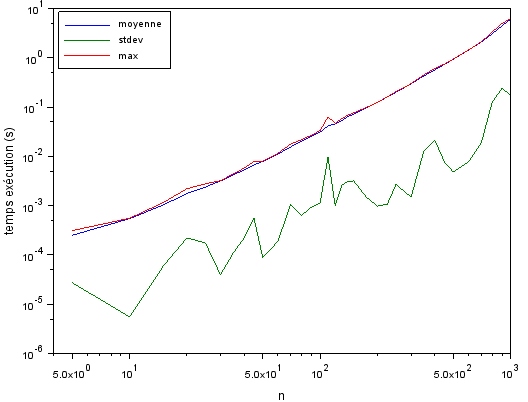
\includegraphics[scale=0.80]{time_LDLt}
\end{figure}
Dans un graphique \(\log\log\), les fonctions \(x^k\) apparaissent comme des droites de pente \(k\). Ici la courbe de la moyenne à une pente d'environ \(2\), ce qui est significativement moins que la valeur théorique \(\mathcal{O}(n^3)\). C'est très certainement dû aux optimisations de \texttt{BLAS/LAPACK}, cependant on remarque que la courbe n'est pas tous à fait linéaire, vers les grandes valeur de \(n\) la pente devient supérieur à \(2\).

On compare \(LDL^t\) et \(LU\) (sans pivot partiel) avec la fonction \texttt{myldlt.sci: comp\_mylu\_myldlt()}

\begin{table}[H]
\centering
\renewcommand*\arraystretch{1.3}
\caption{Comparaison \(LDL^t\ -\ LU\)}
\begin{tabular}{|l|c|c|c|}
  \hline
  n & erreur & temps exécution \(LDL^t\) (s) & temps exécution \(LU\) (s) \\
  \hline
	5	&	\(5.81 \times 10^{-16}\)	&	\(2.69 \times 10^{-4}\)	&	\(1.83 \times 10^{-4}\) \\
	10	&	\(2.18 \times 10^{-15}\)	&	\(6.58 \times 10^{-4}\)	&	\(3.21 \times 10^{-4}\) \\
	25	&	\(1.21 \times 10^{-14}\)	&	\(2.47 \times 10^{-3}\)	&	\(9.59 \times 10^{-4}\) \\
	50	&	\(3.64 \times 10^{-14}\)	&	\(8.24 \times 10^{-3}\)	&	\(2.75 \times 10^{-3}\) \\
	100	&	\(1.39 \times 10^{-13}\)	&	\(3.04 \times 10^{-2}\)	&	\(1.23 \times 10^{-2}\) \\
	200	&	\(5.66 \times 10^{-13}\)	&	\(1.27 \times 10^{-1}\)	&	\(7.22 \times 10^{-2}\) \\
	300	&	\(1.62 \times 10^{-12}\)	&	\(2.99 \times 10^{-1}\)	&	\(2.19 \times 10^{-1}\) \\
	500	&	\(3.98 \times 10^{-12}\)	&	\(9.47 \times 10^{-1}\)	&	\(1.21\) \\
	750	&	\(8.12 \times 10^{-12}\)	&	\(2.69\)				&	\(4.88\) \\
	1000 &	\(1.54 \times 10^{-11}\)	&	\(6.61\) 				&	\(12.8\) \\
  \hline
\end{tabular}
\caption*{\textit{L'erreur est la 2-norme de la différence entre \(LDL^t\) et \(LU\)}}
\end{table}

On remarque que sur de petite matrice \(LU\) est plus rapide, mais que sur de grande matrice c'est \(LDL^t\) qui est plus rapide. L'algorithme \(LU\) a une complexité du même ordre que \(LDL^t\) mais il fait un peu plus de calculs dans la boucle principale :  \begin{minted}{scilab}
// boucle principale LU
A(k+1:n, k+1:n) = A(k+1:n,k+1:n) - A(k+1:n,k) * A(k,k+1:n)
// boucle principale LDLt
A(j+1:n,j) = (A(j+1:n,j) - A(j+1:n,1:j-1) * v(1:j-1))/A(j,j)
\end{minted}
On peut expliquer que notre algorithme \(LU\) est plus rapide sur de petites valeurs de \(n\) par sa compacité. Il n'y a qu'une boucle et on utilise presque exclusivement les opérations vectorielles de \texttt{scilab}, le code est fortement optimisé, mais ça ne suffit pas pour battre \(LDL^t\) sur de grandes matrices.

\section{CSR}

Pour implémenter un algorithme de multiplication d'une matrice creuse au format CSR, on regarde comment se présente une matrice CSR.

Soit \(A\) une matrice creuse, tel que :
\[
A = 
\begin{pmatrix}
	0	&	0	&	0	&	0	& 0	\\
	0	&	9	&	13	&	0	& 0	\\
	0	&	0	&	0	&	11	& 0	\\
	12	&	0	&	0	&	0	& 0	\\
	0	&	0	&	0	&	0	& 9	\\
	0	&	3	&	0	&	0	& 0	\\
	5	&	0	&	0	&	0	& 0	\\
\end{pmatrix}
\]

Au format CSR, elle se présente sous cette forme :
\[
\texttt{AA}  = 
\begin{bmatrix}
9	&	13	&	11	&	12	&	9	&	3	&	5	\\
\end{bmatrix}
\]
\[
\texttt{JA}  = 
\begin{bmatrix}
2	&	3	&	4	&	1	&	5	&	2	&	1	\\
\end{bmatrix}
\]
\[
\texttt{IA}  = 
\begin{bmatrix}
1	&	1	&	3	&	4	&	5	&	6	&	7	&	8	\\
\end{bmatrix}
\]

\texttt{AA} contient les valeurs, \texttt{JA} le numéro de la colonne de la valeur associer, et \texttt{IA} l'index des sauts de lignes (index des éléments \texttt{AA} et \texttt{JA}). \texttt{IA} commence toujours par 1, lorsqu'une ligne est sauté (ligne de 0) l'index est répété dans \texttt{IA}, par exemple ici : la première ligne est sauté, donc après le premier \(1\) obligatoire, on met un second \(1\).

On remarque qu'au format CSR, la taille du vecteur \texttt{IA} est la même que celle du \texttt{nombre de lignes + 1}, le vecteur de sorti du produit \(Ax\) aura donc un nombre d'élément égal à \texttt{length(IA)-1}

Soit \(x\) un vecteur, on souhaite faire le produit matrice vecteur \(Ax\), le vecteur x soit avoir le même nombre d'élément que le nombre de colonne de \(A\).
La boucle principale de l'algorithme de multiplication CSR doit se faire sûr le nombre d'élément non nul de A, à l'intérieur de celle ci on place une boucle while qui incrémentera l'indicateur de la ligne actuelle tant que \texttt{IA} nous dit de sauter de ligne. Le produit scalaire se fait élément par élément, l'élément \texttt{AA(i)} est positionner à la colonne \texttt{JA(i)} donc on sait par quel élément de \(x\) on doit le multiplier \texttt{x(JA(i))}. La complexité de l'algorithme est en \(\mathcal{O}(\texttt{nombre\ éléments\ non\ nul})\).

\begin{scriptsize}
\centering
\begin{minted}{scilab}
function [v] = csr_mv(AA, JA, IA, x)
    n = length(JA)
    v = zeros(length(IA)-1,1)
    k = 1 // ligne actuelle
    for i=1:n
        while(i == IA(k+1)) // saute les lignes nulles
            k = k + 1
        end
        v(k) = v(k) + AA(i) * x(JA(i))
    end
    if(isrow(x)) // col/row coherente avec x
        v = v'
    end
endfunction
\end{minted}
\end{scriptsize}

Pour tester cet algorithme, on a besoin de pouvoir générer des matrices creuses, et calculer leur forme CSR.

Un moyen efficace pour généré des matrices creuse est de remplir une matrice vide de quelques valeurs aléatoires, puis de permuter aléatoirement ses éléments. Pour cela on utilise la fonction \texttt{grand(1, "prm", A)} de \texttt{scilab}, le \texttt{"prm"} signifie qu'on souhaite une permutation, le 1 signifie que l'on en veut qu'une seule, et \texttt{A} est la matrice à permuter. Voir l'implémentation dans \texttt{csr.sci: make\_mat\_creuse(..)}
\newline\indent

L'algorithme pour calculer le format CSR est aussi très simple. On parcours \(A\) avec deux boucle fort (selon les lignes), on note les valeurs non nulle dans \texttt{AA}, les colonnes dans \texttt{JA}, et lorsqu'on change de ligne on mets d'indice dans \texttt{IA}. Cependant étant donné qu'on doit parcourir toutes les cases de \(A\), cet algorithme est en \(\mathcal{O}(n^2)\). Voir l'implémentation dans \texttt{csr.sci: make\_csr(A)}.

On peut tester cet algorithme en faisant et défaisant la forme CSR (avec la fonction \texttt{csr.sci: undo\_csr(..)}), puis en prenant la 2-norme de la matrice initiale moins celle qui a été fait puis défait. On trouve que ces matrices sont toujours identique quelque soit la taille de la matrices initiale. Voir l'implémentation dans \texttt{csr.sci: test\_csr()}
\newline\indent

On peut maintenant tester la multiplication matrice creuse vecteur. On génère d'abord une matrice creuse \texttt{n}\(\times\)\texttt{m} avec la fonction \texttt{make\_mat\_creuse}, on génère aussi un vecteur creux \texttt{m}\(\times\)\texttt{1} avec la même fonction. On converti cette matrice en CSR avec \texttt{make\_csr}, puis on récupère le vecteur sortie de \texttt{csr\_mv} que l'on compare avec \(Ax\) (en prenant la 2-norme de la différence). Voir l'implémentation dans \texttt{csr.sci: test\_csr\_mv()}

Même pour des matrices très grande (\(5000\times3000\)), la différence entre les solutions est toujours nulle. L'algorithme \texttt{csr\_mv} donne donc un résultat correct.

On peut comparer les performances de \texttt{csr\_mv} avec \texttt{Ax}. Pour de grandes matrices, la majorité du temps est perdu en calculant le format CSR avec la fonction \texttt{make\_csr} (qui est en \(\mathcal{O}(n^2)\)). 

\begin{table}[H]
\centering
\caption{Comparaison \texttt{csr\_mv - Ax}}
\renewcommand*\arraystretch{1.3}
\begin{tabular}{|l|c|c|c|}
  \hline
  n\(\times\)m & temps exécution \texttt{csr\_mv} (s) & temps exécution \(Ax\) (s) \\
  \hline
	\(5 \times 5\)		&	\(6.62 \times 10^{-5}\)	&	\(3.80 \times 10^{-6}\)	\\
	\(25 \times 25\)	&	\(4.63 \times 10^{-4}\)	&	\(4.60 \times 10^{-6}\)	\\
	\(75 \times 40\)	&	\(1.79 \times 10^{-3}\)	&	\(6.10 \times 10^{-6}\)	\\
	\(100 \times 100\)	&	\(5.64 \times 10^{-3}\)	&	\(1.06 \times 10^{-5}\)	\\
	\(500 \times 325\)	&	\(9.88 \times 10^{-2}\)	&	\(1.37 \times 10^{-4}\)	\\
	\(2500 \times 1200\)&	6.08					&	\(2.14 \times 10^{-3}\)	\\
	\(5000 \times 3000\)&	29.0					&	\(1.07 \times 10^{-2}\)	\\
  \hline
\end{tabular}
\caption*{\textit{On vérifie systématiquement que les deux vecteurs résultats sont identiques.}}
\end{table}

On remarque que le produit matrice vecteur natif de \texttt{scilab} est dans tous les cas plus performant, que notre \texttt{csr\_mv}. Notre fonction est interprété par \texttt{scilab} c'est ce qui fait qu'elle est moins performante. Dans un langage compilé comme C, le produit matrice vecteur CSR serait plus rapide que le produit matrice vecteur classique.

\section{Poisson 1D}

\textcolor{red}{TODO: Raconter vite fais le cours/td}
\textcolor{red}{TODO: C}

\begin{minted}{scilab}
function [] = test_myldlt()
\end{minted}


\end{document}
